% Template for a Computer Science Tripos Part II project dissertation
\documentclass[12pt,a4paper,twoside,openright]{report}
\usepackage[pdfborder={0 0 0}]{hyperref}    % turns references into hyperlinks
\usepackage[margin=25mm]{geometry}  % adjusts page layout
\usepackage{graphicx}  % allows inclusion of PDF, PNG and JPG images
\usepackage{verbatim}
\usepackage{docmute}   % only needed to allow inclusion of proposal.tex
\usepackage{tabularx}
\usepackage{listings}
\usepackage{minted}
\usepackage[english]{babel}
\usepackage{blindtext}
\lstset{
basicstyle=\small\ttfamily,
breaklines=true
}

\raggedbottom                           % try to avoid widows and orphans
\sloppy
\clubpenalty1000%
\widowpenalty1000%

\renewcommand{\baselinestretch}{1.1}    % adjust line spacing to make
                                        % more readable

\begin{document}

\bibliographystyle{plain}


%%%%%%%%%%%%%%%%%%%%%%%%%%%%%%%%%%%%%%%%%%%%%%%%%%%%%%%%%%%%%%%%%%%%%%%%
% Title


\pagestyle{empty}

\rightline{\LARGE \textbf{Jacob Fenton}}

\vspace*{60mm}
\begin{center}
\Huge
\textbf{Efficient Asymmetric Cryptography for RFID Access Control} \\[5mm]
Computer Science Tripos -- Part II \\[5mm]
Fitzwilliam College \\[5mm]
\today  % today's date
\end{center}

%%%%%%%%%%%%%%%%%%%%%%%%%%%%%%%%%%%%%%%%%%%%%%%%%%%%%%%%%%%%%%%%%%%%%%%%%%%%%%
% Proforma, table of contents and list of figures

\pagestyle{plain}

\chapter*{Proforma}

{\large
\begin{tabularx}{\linewidth}{l X}
Name:               & \bf Jacob Fenton                       \\
College:            & \bf Fitzwilliam College                     \\
Project Title:      & \bf Efficient Asymmetric Cryptography for RFID Access Control \\
Examination:        & \bf Computer Science Tripos -- Part II, 2018  \\
Word Count:         & \bf TODO  \\
Project Originator: & Dr Markus Kuhn                    \\
Supervisor:         & Dr Markus Kuhn                    \\ 
\end{tabularx}
}

\section*{Original Aims of the Project}

The objective of the project was to produce an access control system that implements an authentication protocol based on asymmetric key cryptography. As well as producing a card application and reader application that implement the authentication protocol, a card-provisioning application that can be used to issue new cards or reprogram existing cards was to be written. The system was required to be able to authenticate a card in less than one second.

\section*{Work Completed}

I have devised and implemented a basic authentication protocol, which includes writing applications to run on both the card and the reader. This basic protocol is able to authenticate a card in under one second, as specified by the success criteria in the project proposal\footnote{See \autoref{appendix:proposal}.}. As an extension, I've also implemented a more advanced protocol based on the Open Protocol for Access Control Identification and Ticketing with PrivacY (OPACITY) \cite{OPACITY} with Full Secrecy (FS), which provides user untraceability and mutual authentication. Finally, I've written the command-line card-provisioning application, which is used for (re)programming cards.

\section*{Special Difficulties}

None.
 
\newpage
\section*{Declaration}

I, Jacob Fenton of Fitzwilliam College, being a candidate for Part II of the Computer
Science Tripos, hereby declare that this dissertation and the work described in it are my own work,
unaided except as may be specified below, and that the dissertation
does not contain material that has already been used to any substantial
extent for a comparable purpose.

\bigskip
\leftline{Signed Jacob Fenton}

\medskip
\leftline{Date \today}

\tableofcontents

\listoffigures

\listoflistings

\newpage

%%%%%%%%%%%%%%%%%%%%%%%%%%%%%%%%%%%%%%%%%%%%%%%%%%%%%%%%%%%%%%%%%%%%%%%
% now for the chapters

\pagestyle{headings}

\chapter{Introduction}

\section{Smart-cards}

In recent years, contactless smart-cards (also known as integrated circuit cards, or ICCs) have become extremely popular for a great number of applications. Perhaps one of the first major applications was by Transport for London, whereby contactless ``Oyster cards'' could be used in place of paper tickets for travel on buses and the underground railway system. As they've become more affordable and the development ecosystem has expanded, their use has become even more widespread. In the UK, contactless bank cards\footnote{Strictly speaking, these are dual interface cards, as they have an electrical contact located on the outside of the card which can be used for a hard connection, as well as the internal antenna which allows for contactless communication.} are commonplace, and the University of Cambridge distributes contactless university cards to students, which can be used to gain access to colleges/departments. Some colleges even allow students to pay for food and drink with these cards.

Contactless smart-cards come in two kinds: memory cards and microprocessor cards. Both types have an antenna and some form of memory, with microprocessor cards also having a CPU. Thus, memory cards have no ability to process data on-card. Neither type of card has a battery. Instead, the card is powered by the card reader through radio-frequency induction. As a result, smart-cards are very low power and complex computations take significantly longer than they would on an inexpensive laptop or phone. Communication between the card and card reader also occurs over radio frequency.

\section{MIFARE Classic}

The current University of Cambridge access control system is based on the MIFARE Classic smart-card, a memory smart-card which conforms to ISO 14443-A \cite{ISO14443}, a standard for contactless ICCs to communicate with a ``coupling device'' (i.e. a smart-card reader) over radio frequency. There are huge numbers of this particular card in existence --- over 200 million are in use today.

The cryptographic protocol used in the card, a scheme named CRPYTO-1, was developed in-house by the manufacturer of the MIFARE Classic, NXP Semiconductors. NXP chose to keep the scheme secret, a practice known as security by obscurity. Such practice is eschewed by the security community because naturally, all cryptographic schemes are bound to have weaknesses, and if researchers (or others) are not able to analyse a scheme, these weaknesses will likely go unnoticed, leaving them open to exploitation by anyone without pure intentions. Furthermore, obscurity does not prevent others from deducing the details of the scheme by observing it in operation and indeed this was the case for CRYPTO-1. In December 2007, a presentation at the Chaos Communication Congress (an annual security conference) by two German researchers, Nohl and Pl{\"o}tz, described a partial reverse engineering of CRYPTO-1, as well as some weaknesses. They managed to do this by reconstructing the card's electronic circuit from photos of the chip. They then verified their reconstruction by eavesdropping on the reader-card communication. Just a few months later, in March 2008, researchers in the Digital Security group at Radboud University Nijmegen revealed a complete reverse engineering of the scheme and were able to clone and manipulate the contents of a MIFARE Classic card. The most serious attack they detailed in their paper can recover the card's cryptographic key in under a second using only a laptop, without any pre- computation.

\subsection{Use of Symmetric Key Cryptography}

Ignoring the fact that the CRYPTO-1 scheme is inherently flawed, NXP's choice to use symmetric key cryptography for the MIFARE Classic was perhaps a misstep. Symmetric ciphers utilize what is called a shared secret, or secret key. Two parties wanting to communicate will first exchange this key over a secure channel and then use it to encrypt/decrypt messages sent between them. In the case of access control cards, this means that a card will store just one key, its own secret key, but that key will be stored in every door reader to which the card has access. This means that if a door reader is compromised, and the attacker is able to retrieve all the keys stored within, then they're able to clone any card which had access to that door. If this door is not in a very specific department, then many people will have access to it, and thus the attacker will have access to a very diverse set of doors --- essentially, the entire system is compromised.

Such a weakness does not exist when using a scheme based on asymmetric key cryptography, in which each card has not one but two keys --- one public, one private. The private key is known only to the owner and is never sent over any channel, whilst the public key is known to everyone. If two parties wish to communicate, then they encrypt their messages with each other's public keys. The message can now only be decrypted with the recipient's private key, which only the recipient knows. In this case, the door reader contains only a long list of public keys corresponding to all the cards that can access the door. Thus, an attacker who's able to compromise a reader doesn't learn any secret information except for the door's private key. This only allows them to clone that specific door reader and doesn't compromise any other cards or readers in the system.

The tradeoffs here are as follows:

\begin{itemize}
\item Symmetric key cryptography is computationally much more simple and, therefore quicker than asymmetric key cryptography.
\item Symmetric key cryptography involves \emph{shared} secrets, meaning a wider potential attack vector and more vulnerable system than one using asymmetric key cryptography.
\end{itemize}

\subsection{Memory Structure}

Before discussing the vulnerabilities of MIFARE Classic, it helps to understand the memory structure. Memory is divided into data blocks of 16 bytes, with blocks being grouped into sectors. The first block of the first sector contains special read-only data. The first 4 bytes contain the unique identifier of the card (UID), followed by a 1-byte \emph{bit count check} (BCC). The rest of the block stores manufacturer-specific data.

The last data block in every sector, known as the \emph{sector trailer}, contains two secret keys A and B which are used for authenticating to a sector. Once authenticated to a sector, the card reader may perform operations on it, depending on the \emph{access conditions} which are also defined in the sector trailer. Access conditions are defined for both keys, to allow different levels of access depending on which key is used for authentication, e.g. key A may have read/write permissions whilst key B may only have read permissions. A diagram of the memory structure of a MIFARE Classic card is shown in \autoref{mifarememory1}.

\begin{figure}[tbh]
\centerline{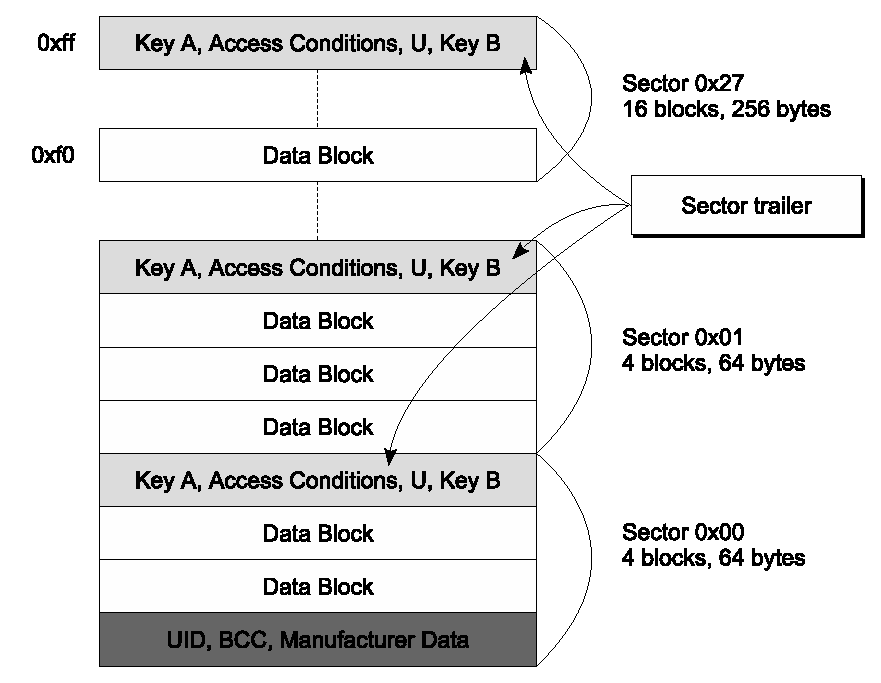
\includegraphics{figures/mifarememory1.eps}}
\caption{MIFARE Classic memory organisation}
\label{mifarememory1}
\end{figure}

The sector trailer itself has specific access conditions. Key A is never readable and key B can be configured to be readable or not. In the latter case, the sector is used just for data storage and only key A can be used to authenticate to the sector. Besides the keys and access conditions, there's one data byte (U) remaining, which has no defined purpose. A diagram of the sector trailer is shown in \autoref{mifarememory2}.

\begin{figure}[tbh]
\centerline{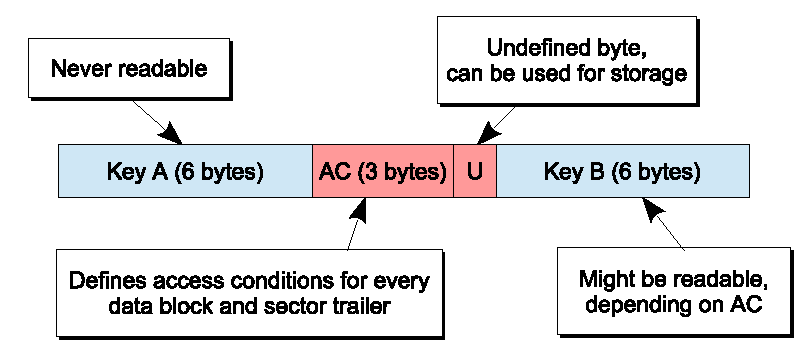
\includegraphics{figures/mifarememory2.eps}}
\caption{Sector trailer}
\label{mifarememory2}
\end{figure}

\subsection{Vulnerabilities}

A number of weakness and vulnerabilities have been discovered in the MIFARE Classic system, including brute-forcible keys, a predictable pseudo-random number generator (PRNG), a cloning attack, and two very powerful attacks named the nested authentication attack and the Dark-Side attack. We shall discuss these vulnerabilities in the following paragraphs.

\subsubsection{Brute-forcing the sector keys}

As stated above, sector keys (A and B) are only 48 bits long, meaning they're vulnerable to a brute-force attack. This involves trying all $2^{48}$ possible keys one-by-one until the correct key is found. It has been shown that this can be done on dedicated hardware\footnote{FPGAs or GPUs.} in a matter of hours \cite{mifarebruteforce}.

\subsubsection{Predicting the output of the card's PRNG}

A PRNG is supposed to generate a sequence of numbers that are effectively indistinguishable from random or, put another way, an adversary should not be able to guess the next number in the sequence. In MIFARE Classic, the on-card PRNG plays an important role in the sector authentication protocol, CRYPTO-1. Specifically, it turns out that if we can predict the output of the PRNG, we're able to authenticate to sectors for which we do not know either of the keys --- this is the nested authentication attack, which is explained in the next paragraph. It was discovered that the output of the MIFARE Classic PRNG depends only on the amount of time that has elapsed since the card was powered up by the reader and that the PRNG has a period of 0.618s. Thus, its output is entirely predictable, making the following attack possible.

\subsubsection{Nested authentication attack}

This attack allows an adversary to obtain all the keys for every sector on the card if just one key (A or B) is known for any sector. A readily available list of known default keys for MIFARE Classic cards exists and, unfortunately, many systems do not update these keys before issuing cards. When testing my own University of Cambridge card, I discovered that five default keys were in use.

When a reader attempts to authenticate to a sector on a card, the card produces a nonce, generated by the weak on-card PRNG, which it sends to the reader. Both the card and reader then derive some key stream bits using this nonce and the key for the sector (one of A or B). The trick here is that, once the reader has authenticated to a sector, subsequent authentication requests are encrypted. Furthermore, upon receiving an authentication request for a new sector, the card sets the internal state of the cipher to the key for the new sector. Thus, when the card sends the \emph{encrypted} nonce for a subsequent authentication request, since we are able to predict the nonce value, we can discover the key stream bits --- the first 32 bits of the sector key --- used to encrypt it by XORing the encrypted nonce with our prediction. Now we can easily brute-force the last 16 bits of the key.

\subsubsection{Dark-Side attack}

This attack allows an adversary to recover any key for any sector without any prior knowledge of any keys. During the authentication protocol, there's a single step where the reader sends encrypted data to the card, along with 8 parity bits. Parity bits are used in communication as a method for error detection/correction. It was noticed that if random data was sent by the reader, then with probability $1/256$, the card will respond in an unexpected way. The reason for this is that if any parity bits are wrong, the card won't respond at all. However, if all the parity bits are correct, but the corresponding data sent by the reader is not correct\footnote{The details of what a ``correct'' response is are specific to the authentication protocol. See \cite{darkside} for more information.}, the card responds with a 4-bit error code, 0x5 (NACK), which is encrypted. Since the plaintext is known, the attacker can recover the four key stream bits used to encrypt the NACK. By repeating this procedure many times, the internal state of the cipher can be discovered, allowing the attacker to completely reconstruct the sector key.

\subsubsection{Combined attack}

The combination of the nested authentication and Dark-Side attacks allows an adversary to completely recover all the keys from any card. They can first run the nested attack to determine if any default keys are in use. If this is not the case, they instead run the Dark-Side attack to recover just one key for any sector. With this one key, they can then rerun the nested attack to recover all other keys.

\subsubsection{Cloning cards}

Once all the keys have been recovered from a card, all the data can be read from it and written to another card, producing a clone. There's one slight issue here, however. As mentioned earlier, the first block of the first sector of a MIFARE Classic card contains a special piece of \textbf{read-only} data --- the UID. On legitimate MIFARE Classic cards, this value is burned onto the card during manufacturing, and is indeed unchangeable. However, there exist unofficial cards which emulate the MIFARE Classic system and have a programmable UID.\footnote{Such as the Fundan Microelectronics FM11RF08.} With one of these cards, an adversary is able to create an exact clone of any legitimate card.

\chapter{Preparation}

\section{Starting point}

This project makes significant use of the material from Security I and Security II. Further, material from Object-Oriented Programming and Further Java was utilised when writing the smart card application that runs on the JavaCard platform, which supports a subset of the Java language.

A previous attempt was made at this project by Denys Natykan, and so his dissertation deserves mention. However, there're rather significant differences in our end products, as I opted to implement a different authentication protocol in order to complete certain extensions.

\section{Communication between card and reader}

The format for communication between a card and a reader is defined by ISO 7816-4 \cite{ISO78164}. It states that the basic unit of communication is the application protocol data unit (APDU). There are two categories of APDUs: commands APDUs and response APDUs. The reader is always the party that initiates communications and thus only ever sends command APDUs. Correspondingly, the card always waits for commands from the reader and thus only ever sends response APDUs.

\subsection{Command APDU}

Command APDUs consist of a required 4-byte header and an optional body. The header contains the following four elements, each 1-byte long:

\begin{itemize}
\item CLA --- indicates the class of command, interindustry or proprietary.
\item INS --- instruction code, indicates the specific command, e.g. ``initiate authentication''.
\item P1, P2 --- instruction parameters, these are command specific.
\end{itemize}

\noindent
The optional body contains the following three elements:

\begin{itemize}
\item L\textsubscript{c} --- a single byte encoding the number (N\textsubscript{c}) of bytes of command data to follow.
\item Command data --- N\textsubscript{c} bytes of data.
\item L\textsubscript{e} --- a single byte encoding the maximum number (N\textsubscript{e}) of response bytes expected.
\end{itemize}

\noindent
If the body is included, parts can be left out depending on the requirements, e.g. if the command has no data, but a response is expected, only the L\textsubscript{e} field will be present. Similarly, if the command has data but doesn't expect a response, only the L\textsubscript{c} and command data fields will be present. A diagram of the structure of a command APDU is shown in \autoref{commandapdu}.

\begin{figure}[tbh]
\centerline{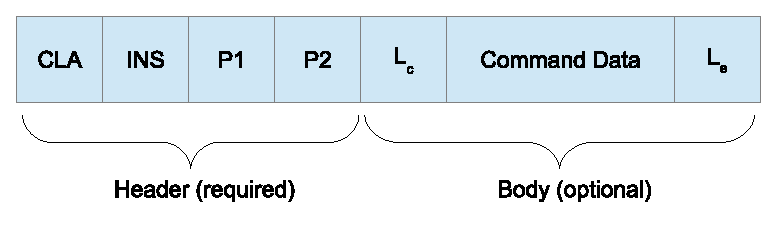
\includegraphics{figures/commandapdu.eps}}
\caption{Command APDU}
\label{commandapdu}
\end{figure}

\subsection{Response APDU}

Response APDUs consist of an optional body and a required 2-byte trailer. The optional body contains any response data the card wishes to send to the reader, and should not exceed N\textsubscript{e} bytes in length. The trailer contains two \emph{status word} bytes, SW1 and SW2, which indicate the command processing status (e.g. 0x9000 indicates no error, command success, whereas 0x6A80 indicates wrong data). A diagram of the structure of a response APDU is shown in \autoref{responseapdu}.

\begin{figure}[tbh]
\centerline{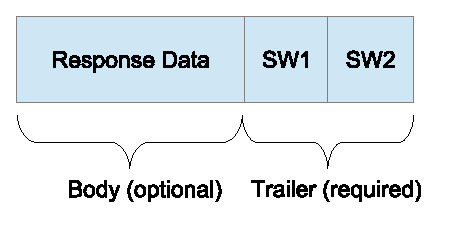
\includegraphics{figures/responseapdu.eps}}
\caption{Response APDU}
\label{responseapdu}
\end{figure}

\section{JavaCard}

The JavaCard platform allows Java-based applets to be run securely on smart-cards with limited memory and processing capabilities. The choice to use a smart-card that implemented JavaCard was made for a few reasons. Firstly, the development ecosystem is very mature --- Oracle make available extensive documentation and resources, perhaps most importantly of which are detailed API references. One article in particular was an excellent introduction to writing JavaCard applets \cite{writingapplets}. There's also an active development community, and I was able to find solutions to many of the problems that arose during the implementation stage by searching forums.\footnote{E.g. https://www.javacardos.com/javacardforum and Stack Overflow.} Because of the fact that JavaCard uses a subset of the Java language, there's no chance for security vulnerabilities resulting from pointer arithmetic. JavaCard also makes extending a card's functionality very simple, as multiple applets can be deployed on a card and new applets can be installed even after a card has been issued.

\subsection{Language}

The JavaCard Virtual Machine (JCVM) specification defines an allowed subset of the Java programming language. Perhaps one of the biggest differences is that only the \texttt{boolean}, \texttt{byte} and \texttt{short} types are permitted --- support for \texttt{int} is optional, and the card I used for this project didn't support it. Further, JavaCard does not require a garbage collector and so one may not assume that objects which are allocated are ever deallocated. A further discussion of memory occurs in \autoref{javacardmemory}. Multi-threading is not supported; although multiple applets can reside on a card, only one can be active at any one time.

\subsection{JavaCard Virtual Machine}

The VM for the JavaCard platform is implemented in two parts, with one part external to the card and the other running on the card itself. The on-card VM interprets bytecode, manages classes and objects, and so on. The external part, referred to as the \emph{converter tool}, loads, verifies, and further prepares the Java classes in a card applet for on-card execution. The output of the converter tool is a Converted Applet (CAP) file, a file that contains all the classes in a Java package in a loadable, executable binary representation. The converter verifies that the classes conform to the Java Card specification. The CAP file can then be installed onto a card.

\begin{figure}[tbh]
\centerline{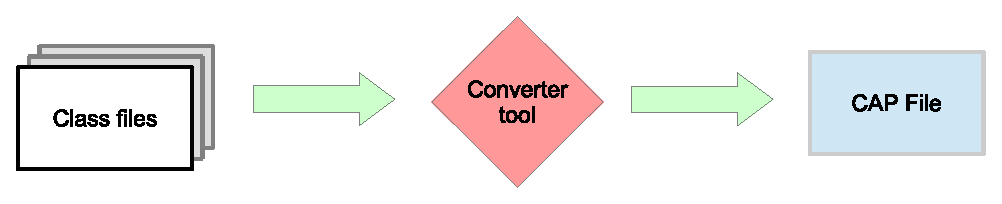
\includegraphics{figures/capconverter.eps}}
\caption{CAP Converter Tool}
\label{capconverter}
\end{figure}

\subsection{Applets}

Applications that run on the card are called applets. Each applet on the card must be uniquely identified by an Application ID (AID). An AID, as defined in ISO 7816-5 \cite{ISO78165}, is a sequence of between 5 and 15 bytes. All applets must extend the \texttt{javacard.framework.Applet} abstract base class.

\subsubsection{Applet life-cycle}

The applet life-cycle begins when the applet is downloaded to the card and the JavaCard Runtime Environment (JCRE) invokes the applet's static \texttt{Applet.install()} method, and the applet registers itself with the JCRE by invoking \texttt{Applet.register()}. Once the applet is installed and registered, it is in the unselected state, available for selection and APDU processing. While in the unselected state, the applet is inactive. An applet gets selected for APDU processing when the host application asks the JCRE to select a specific applet in the card (by instructing the card reader to send a \texttt{SELECT} APDU). To notify the applet that a host application has selected it, the JCRE calls its \texttt{select()} method; the applet typically performs appropriate initialization in preparation for APDU processing.

Once selection is done, the JCRE passes incoming APDU commands to the applet for processing by invoking its \texttt{process()} method.

Applet deselection occurs when the host application tells the JCRE to select another applet. The JCRE notifies the active applet that it has been deselected by calling its \texttt{deselect()} method, which typically performs any clean-up logic and returns the applet to the inactive, unselected state. If power is lost, the applet is reset to the inactive state without the \texttt{deselect()} method being called. \autoref{appletlifecycle} summarises the applet life-cycle.

\begin{figure}[tbh]
\centerline{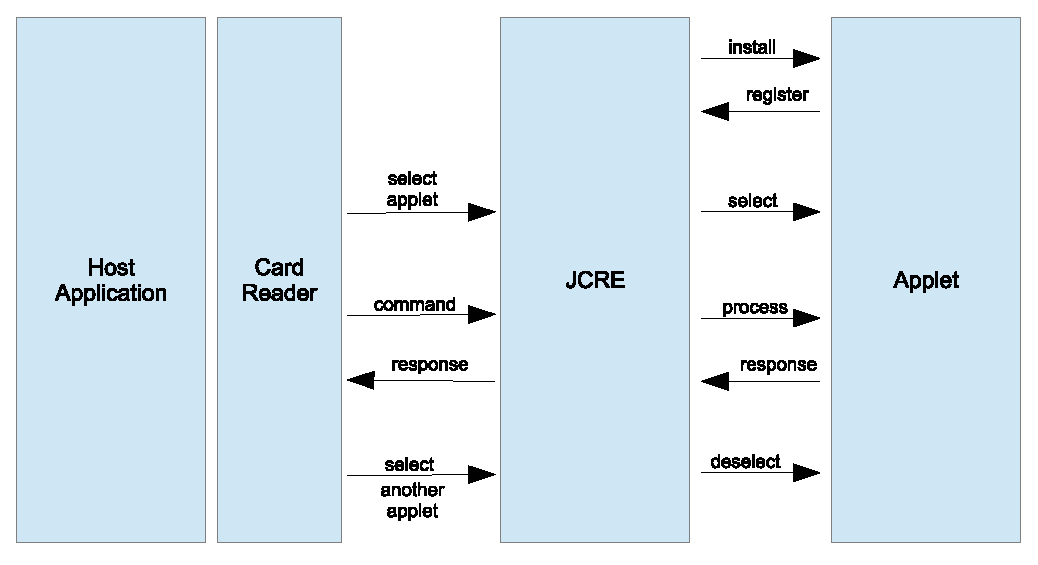
\includegraphics{figures/appletlifecycle.eps}}
\caption{Applet Life-Cycle}
\label{appletlifecycle}
\end{figure}

\subsection{Memory organisation} \label{javacardmemory}

JavaCard smart-cards offer two types of memory: transient Random Access Memory (RAM) and persistent Electronically Erasable Programmable Read-Only Memory (EEPROM). Typically, much more EEPROM than RAM memory is available --- the NXP J3A040 has 40KB of EEPROM but roughly 6KB of RAM. However, RAM read/write speeds are faster by an approximate factor of $10^3$.

\subsubsection{Transient RAM}

Transient memory is erased on power down and is thus only suitable for storing temporary data. As an example, during execution of my OPACITY-FS inspired protocol, several encryption keys must be derived using a key derivation function (KDF). These keys are only needed for the duration of the protocol execution, and thus do not need to persist when the card loses power. Therefore, it would be perfectly suitable to use transient buffers to hold them. Transient objects can only be created via the JavaCard API, e.g. to create a transient byte array, one must call \texttt{JCSystem.makeTransientByteArray()}.

Note that, although the actual memory is transient, the reference that points to the memory is persistent. Thus a transient object should only ever be created once, and the ideal place to do this is in the applet's constructor (which should be called by the \texttt{install()} method).

\subsubsection{Persistent EEPROM}

Anytime the \texttt{new} keyword is used, a persistent object will be created. As stated earlier, certain cards do not actually have a garbage collector. Thus it's very important to ensure careful use of EEPROM, since once created, an object may never be erased and memory leaks can easily occur. Writes to EEPROM are atomic, meaning that there's no need for concern over data inconsistencies. Unfortunately, writes also wear out the physical memory circuit, and thus frequent writes will reduce the lifetime of the card.

\section{Resources}



\subsection{Physical resources}

Before I was able to begin the implementation stage, I ordered the following items:

\begin{itemize}
\item Identiv SCL3711 --- A USB smart-card reader. I had originally intended to use this reader, but discovered that, despite the claims of the manufacturer, it was not compatible with my operating system (OSX 10.11, El Capitan).
\item ACS ACR122T --- alternative USB smart-card reader that was compatible.
\item NXP J3A040 CL --- a programmable contactless-only smart-card with 40K of EEPROM memory, implementing JavaCard 2.2.2 and Global Platform 2.1.1, and conforming to ISO 14443-A. I chose this card because it is relatively cheap and it supports many of the cryptographic algorithms that I needed in order to implement an authentication protocol based on asymmetric cryptography\footnote{E.g. support for ECDSA (and AES, which is used in the advanced protocol that I implemented).}. Note that cards may support some algorithms but only for certain key sizes. For example, the J3A040 only supports ECDSA keys of up to 192 bits. Details of what algorithms and key sizes a card supports can be found by using JCAlgTest \cite{jcalgtest}.
\end{itemize}

\subsection{GlobalPlatform and GPShell}

The GlobalPlatform card specification is a standard for the management of the infrastructure of a smart-card, the most relevant tasks being installation and removal of applications on a card. GPShell \cite{gpshell} is a script interpreter used for talking to smart-cards that are compliant with the GlobalPlatform card specification. It can establish a secure channel with a smart-card in order to load, instantiate, delete and list applications on the card. \autoref{gpinstall} shows the script I use to install a CAP file called \texttt{opacity\_fs\_impl.cap} onto a card. The script commands are converted, by GPShell, to command APDUs which are sent to the card via the connected reader.

\begin{lstlisting}[caption={Applet install script},captionpos=b,label={gpinstall}]
enable_trace
establish_context
mode_211
card_connect
select -AID a0000000030000
open_sc -security 1 -keyind 0 -keyver 0
    -mac_key 404142434445464748494a4b4c4d4e4f
    -enc_key 404142434445464748494a4b4c4d4e4f
delete -AID f234123456101000
install -file opacity_fs_impl.cap -sdAID a000000003000000 -priv 2
    -nvDataLimit 5000
card_disconnect
release_context
\end{lstlisting}

\begin{itemize}
\item \texttt{enable\_trace} --- writes a log of all command/response APDUs (hex encoded) to standard output.
\item \texttt{establish\_context} --- before any communication can by done to any card this command must be executed.
\item \texttt{mode\_211} --- sets the protocol mode to GlobalPlatform 2.1.1.
\item \texttt{card\_connect} --- connect to card via reader.
\item \texttt{select -AID a0000000030000} --- select the \emph{card manager} applet. The card manager understands command APDUs for installing/deleting applets. The AID of the card manager is card-specific and may be found in the datasheet.
\item \texttt{open\_sc -security 1 -keyind 0 -keyver 0 -mac\_key 404142434445464748494a4b4c4d4e4f -enc\_key 404142434445464748494a4b4c4d4e4f} --- open a secure channel to the card with the standard JavaCard Open Platform (JCOP) keys; the J3A040 CL is a JCOP card.
\item \texttt{delete -AID f234123456101000} --- delete the applet with the given AID. This was the AID I used for my applet, so this step is just to remove any old version of the applet before installing the new one.
\item \texttt{install -file opacity\_fs\_impl.cap -sdAID a000000003000000 -priv 2 -nvDataLimit 5000} --- install the file named \texttt{opacity\_fs\_impl.cap} and limit its non-volatile (EEPROM) data allowance to 5KB. An option specifies the \emph{security domain} AID (sdAID), which in this case is the card manager.
\item \texttt{card\_disconnect} --- disconnect the card.
\item \texttt{release\_context} --- release the context that was established at the beginning of the script.
\end{itemize}

\subsection{Build tools}

I used Apache Ant \cite{ant} to build all my applications. In combination with a useful Ant task\footnote{https://github.com/martinpaljak/ant-javacard}, I was able to build and convert the card application to a CAP file in one command. The build file I used for the card application can be found in \autoref{appendix:cardappbuildfile}.

\subsection{External libraries}

Four external libraries were used in this project. The first of these was the Apache Commons Codec \cite{apachecommonscodec} library, which was useful because of the \texttt{org.apache.commons.codec.binary.Hex} class, specifically the \texttt{encodeHexString()} method. This allowed me to analyse the card's responses in a readable format and was helpful for debugging. The second was the Bouncy Castle \cite{bouncycastle} library. As well as using it as a provider\footnote{In Java, a ``provider'' implements the Java security API, for instance by providing implementations of cryptographic algorithms (ECDSA, SHA-1) or classes for key generation and management.}, it offered a handful of useful methods that the standard Java API didn't, for example a method for obtaining a byte array of the encoding of a public ECDSA key. The third was the Apache Commons CLI \cite{apachecommonscli} library, which was helpful in parsing flags and arguments passed to the provisioning application. The final library was the JavaCard 2.2.2 SDK.

\chapter{Implementation}

The project consists of three applications: the card-provisioning application, described in \autoref{provisionapp}, and two separate applications that implement the authentication protocol, one that runs on the card, the other on the reader. Two authentication protocols were devised for the project --- the first protocol, described in \autoref{basicauth}, is very basic and only authenticates the card's identity. The second, described in \autoref{mutualauth}, performs mutual authentication and provides user untraceability.

\section{Card-provisioning application}
\label{provisionapp}

Both authentication protocols are built around elliptic curve (EC) cryptography, and thus it was necessary to write a command-line application that provisions cards with a signed EC key pair. The application is also able to list the details stored on a card (CRSID, door access permissions and card expiry date), generate a key pair that it will use for signing card key pairs, and lastly, there's a command for signing a provided file (the reason for this is explained below). \autoref{provisionhelp} shows the help output of the application.

\begin{figure}[tbh]
\centerline{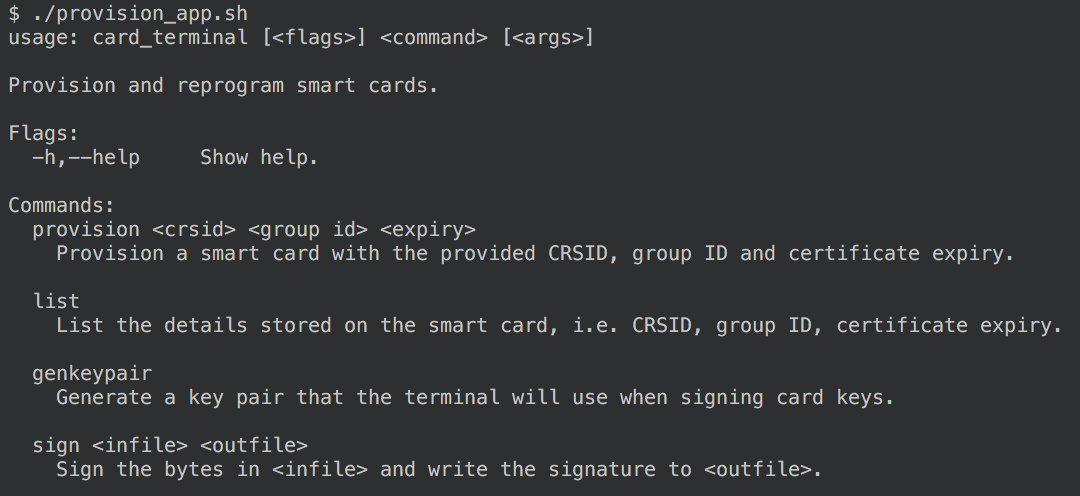
\includegraphics[scale=0.7]{figures/provisionhelp.png}}
\caption{Card-provisioning application help output}
\label{provisionhelp}
\end{figure}

Note that the provision command takes as input three items: CRSID, a \emph{group ID}, and a card expiry date. These items, along with the card's public key, are all included as part of the input data when generating the card's ECDSA signature.

\subsubsection{Card-provisioning terminal key pair}

In order to generate ECDSA signatures, the card terminal needs a key pair of its own. This can be generated using the \texttt{genkeypair} command. It's important that this key pair is kept safe, since all cards and readers contain a copy, in order to perform the mutual authentication protocol. Thus, if it has to be replaced (e.g. if it was accidentally deleted or overwritten), then all cards and readers will have to be re-provisioned.

\subsubsection{Provisioning readers}

In order to perform mutual authentication, readers must also have their own signed EC key pair. The \texttt{sign} command exists for this reason. Once a reader has generated its key pair, the \texttt{sign} command can be called, with the \texttt{<infile>} argument being the reader's public key. Readers also need a copy of the provisioning terminal's public key in order to be able to authenticate card signatures. Both the signature and terminal public key can then be loaded when the reader-side authentication application starts.

\subsection{Format of group ID}

The group ID specifies the access permissions of the card. It is variable-length, and thus no format has been hard-coded into the implementation. One possible option is to have each bit correspond to a certain location. If the bit is set, then the card has access to that location. For example, the sixth bit being set could correspond to permission to access a certain faculty.

\subsection{Card provisioning protocol}

The provisioning protocol is very straightforward. First, the provisioning terminal sends a command APDU to the card telling it to generate an ECDSA key pair. The card replies with a response APDU containing its public key, encoded according to SEC1 \cite{sec1} \S2.3.3. The reader then produces an ECDSA signature, using as input the following items concatenated together in a byte array: CRSID, group ID, card expiry date and card public key. It then sends a \texttt{STORE} command to the card, with the signature, CRSID, group ID, card expiry and its own public key\footnote{As mentioned earlier, the terminal's public key is needed in order for the card to be able to verify a reader's identity during the mutual authentication protocol.} in the body of the APDU. The card copies these items to persistent memory and responds with a ``command success'' status word (0x9000). The reader then sends a \texttt{CHECK} command, where the card returns all the data that it just stored --- this step is to ensure no data corruption occurred. If all the data is correct, the reader sends a final \texttt{LOCK} command, after which the card will not respond to any of the earlier commands until unlocked. A diagram of the provisioning protocol is shown in \autoref{provisioningprotocol}.

\begin{figure}[tbh]
\centerline{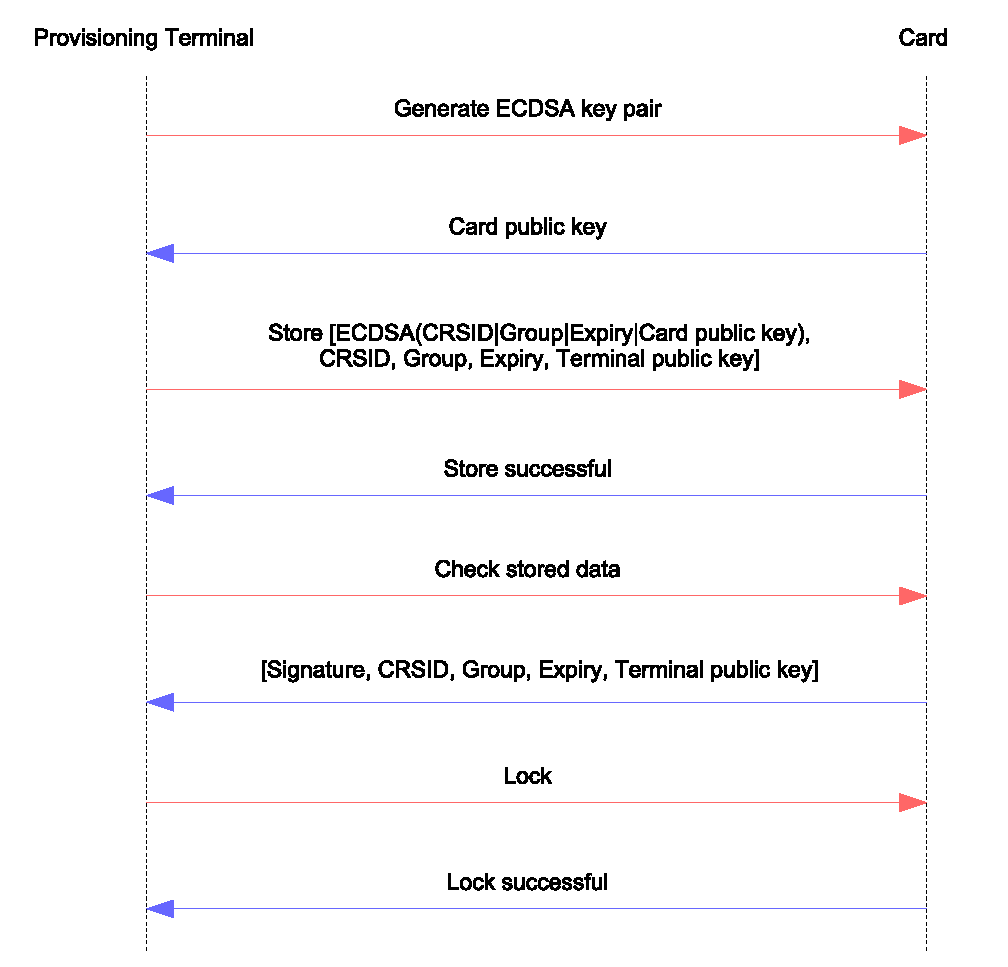
\includegraphics[scale=0.8]{figures/provisioningprotocol.eps}}
\caption{Card-provisioning protocol}
\label{provisioningprotocol}
\end{figure}

\subsubsection{ECDSA signature format}

DER is the data format used to encode an ECDSA signature, which is defined by SEC1 as an ASN.1 sequence of two integers \texttt{r} and \texttt{s}.

\begin{lstlisting}[caption={ASN.1 structure of an ECDSA signature},captionpos=b]
ECDSASignature ::= SEQUENCE {
    r    INTEGER,
    s    INTEGER
}
\end{lstlisting}

\noindent
The following sequence of bytes shows the DER-encoding of an ECDSA signature: \texttt{0x30 b1 0x02 b2 (vr) 0x02 b3 (vs)}.

\begin{itemize}
\item \texttt{0x30} signifies the start of a sequence.
\item \texttt{0x02} signifies the start of an integer.
\item \texttt{b1} is a single byte value, equal to the length, in bytes, of the remaining list of bytes (from the first \texttt{0x02} to the end of the encoding).
\item \texttt{b2} is a single byte value, equal to the length, in bytes, of (vr).
\item \texttt{b3} is a single byte value, equal to the length, in bytes, of (vs).
\item \texttt{(vr)} is the signed, big-endian encoding of the value \texttt{r}, of minimal length.
\item \texttt{(vs)} is the signed, big-endian encoding of the value \texttt{s}, of minimal length.
\end{itemize}

\noindent
\emph{Minimal length} means that the total length is the shortest possible to represent the value, and \emph{signed} means that the first bit of the first byte specifies the sign of the value. Since \texttt{r} and \texttt{s} are always positive, the first bit of the first byte of both \texttt{(vr)} and \texttt{(vs)} must be \texttt{0}, i.e. the first byte must have a value between \texttt{0x00} and \texttt{0x7F}. If the minimal, unsigned representation of either value has a first byte with value greater than \texttt{0x7F}, the encoded representation must be padded with an \texttt{0x00} byte.

The relevance of this is that JavaCard and Bouncy Castle treat signatures slightly differently. JavaCard does not adhere to the ``minimal length'' criteria and always pads \texttt{(vr)} and \texttt{(vs)} with zeros until the signature is the maximum allowed length --- in fact, JavaCard will not be able to decode a signature \emph{unless} it has maximal length. Thus, before sending a signature generated by Bouncy Castle to a card, it must be padded to the maximum length. Equally, when we receive a signature generated by JavaCard, we must remove any incorrectly inserted pads (zeros), else Bouncy Castle will not be able to decode it. This particular issue was extremely difficult to debug.

\section{Basic authentication protocol}
\label{basicauth}

The basic authentication protocol is relatively simple. The reader begins by generating a cryptographic nonce.\footnote{A nonce is a random number, normally used for the purpose of preventing a replay attack.} The reader sends this nonce to the card in the body of a \texttt{BASIC\_AUTH} command. The card generates an ECDSA signature, using the nonce as the input data. It then returns this nonce signature, along with its stored CRSID, group ID, expiry date, EC public key and card signature\footnote{This was the signature stored during provisioning.}, in the body of a response APDU. The reader first verifies the card signature to ensure the card's public key is valid, then checks the card expiry date. Having done that, it verifies the nonce signature to ensure that the card it's communicating with has the matching private key\footnote{Otherwise it's possible that an attacker could just be replaying an old communication; the nonce signature prevents this possibility.}. Finally, the reader checks that the group ID permits access to the location in question. A diagram of the protocol is shown in \autoref{fig:basicauth}.

\begin{figure}[tbh]
\centerline{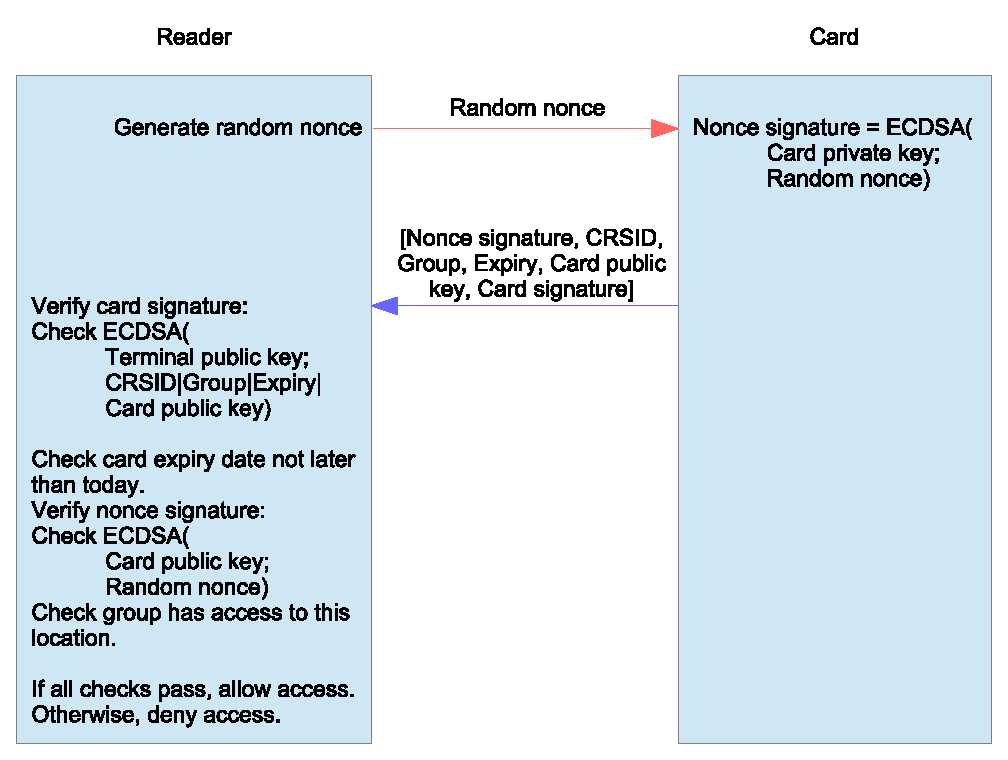
\includegraphics[scale=0.8]{figures/basicauth.eps}}
\caption{Basic authentication protocol}
\label{fig:basicauth}
\end{figure}

\section{Mutual authentication protocol}
\label{mutualauth}

\blindtext

\subsection{Concatenation KDF}

\blindtext

\chapter{Evaluation}



\chapter{Conclusion}


%%%%%%%%%%%%%%%%%%%%%%%%%%%%%%%%%%%%%%%%%%%%%%%%%%%%%%%%%%%%%%%%%%%%%
% the bibliography
\addcontentsline{toc}{chapter}{Bibliography}
\bibliography{refs}

%%%%%%%%%%%%%%%%%%%%%%%%%%%%%%%%%%%%%%%%%%%%%%%%%%%%%%%%%%%%%%%%%%%%%
% the appendices
\appendix

\chapter{Project Proposal}
\label{appendix:proposal}

% Note: this file can be compiled on its own, but is also included by
% diss.tex (using the docmute.sty package to ignore the preamble)
\documentclass[12pt,a4paper,twoside]{article}
\usepackage[pdfborder={0 0 0}]{hyperref}
\usepackage[margin=25mm]{geometry}
\usepackage{graphicx}
\usepackage{parskip}
\begin{document}

\begin{center}
\Large
Computer Science Tripos -- Part II -- Project Proposal\\[4mm]
\LARGE
Efficient Asymmetric Cryptography for RFID Access Control\\[4mm]

\large
J.~Fenton, Fitzwilliam College

Originator: Dr M.~Kuhn

11 October 2017
\end{center}

\vspace{5mm}

\textbf{Project Supervisor:} Dr M.~Kuhn

\textbf{Director of Studies:} Dr R.~Harle

\textbf{Project Overseers:} Dr S.~Holden  \& Dr N.~Krishnaswami

% Main document

\section*{Introduction}

The current university access control system is based on the MIFARE Classic smart card, which conforms to ISO 14443 Type A, a standard for contactless integrated circuit cards to communicate with a ``coupling device'' (i.e. a smart card reader) over radio frequency. There are huge numbers of this particular card in existence --- over 200 million are in use today.

The cryptography used in the card, a scheme named CRYPTO-1, was developed in-house by the manufacturer of the MIFARE Classic, NXP Semiconductors. NXP chose to keep the scheme secret, a practice known as security by obscurity. Such practice is eschewed by the security community because naturally, all cryptographic schemes are bound to have weaknesses and if researchers (or others) are not able to analyse a scheme, then they cannot provide advice as to how flaws within said scheme can be fixed. Furthermore, obscurity does not prevent others from deducing the scheme by observing it in operation and indeed this was the case for CRYPTO-1. In December 2007, a presentation at the Chaos Communication Congress (an annual security conference) by two German researchers, Nohl and Pl{\"o}tz, described a partial reverse engineering of CRYPTO-1, as well as some weaknesses. They managed to do this by reconstructing the card's electronic circuit from photos of the chip. They then verified their reconstruction by eavesdropping on the reader-card communication. Just a few months later, in March 2008, researchers in the Digital Security group at Radboud University Nijmegen revealed a complete reverse engineering of the scheme and were able to clone and manipulate the contents of a MIFARE Classic card. The most serious attack they detailed in their paper can recover the card's cryptographic key in under a second using only a laptop, without any pre- computation. NXP tried to obtain an injunction to prevent publication of the paper but were unsuccessful.

Ignoring the fact that the CRYPTO-1 scheme is inherently flawed, NXP's choice to use symmetric key cryptography for the MIFARE Classic was perhaps a misstep. Symmetric ciphers utilize what is called a shared secret, or secret key. Two parties wanting to communicate will first exchange this key over a secure channel and then use it to encrypt/decrypt messages sent between them. In the case of access control cards, this means that a card will store just one key, its own secret key, but that key will be stored in every door reader to which the card has access. This means that if a door reader is compromised, and the attacker is able to retrieve all the keys stored within, then they're able to clone any card which had access to that door. If this door is not in a very specific department, then many people will have access to it, and thus the attacker will have access to a very diverse set of doors --- essentially, the entire system is compromised. Such a weakness does not exist when using a scheme based on asymmetric key cryptography, in which each card has not one but two keys --- one public, one private. The private key is known only to the owner and is never sent over any channel, whilst the public key is known to everyone. If two parties wish to communicate, then they encrypt their messages with each other's public keys. The message can now only be decrypted with the recipient's private key, which only the recipient knows. In this case, the door reader contains only a long list of public keys corresponding to all the cards that can access the door. Thus, an attacker who's able to compromise a reader doesn't learn any secret information except for the door's private key. This only allows them to clone that specific door reader and doesn't compromise any other cards or readers in the system.

The aim of the project is to produce an access control system that uses asymmetric key cryptography to authenticate smart cards. The system should act as a replacement for the existing MIFARE Classic system.

\section*{Starting point}

The project will make significant use of the material from Security I and Security II --- I have already studied the lecture notes for Security II, although I have set aside some time in my plan for recap. Further, material from Object-Oriented Programming and Further Java will be utilised when writing the smart card application, which runs on the JavaCard platform and supports a subset of the Java language.

A previous attempt was made at this project by Denys Natykan, and so his dissertation must be mentioned as a starting point. However, I already anticipate significant differences between our end products as I intend to use a rather different authentication protocol.

\section*{Substance and structure of the project}

The objective of the project is to produce an access control system that implements an authentication protocol based on asymmetric key cryptography. As well as producing a card application and reader application that implement the authentication protocol, I intend to write a card-provisioning application that can be used to issue new cards or reprogram existing cards.

I intend to compare at least two different digital signature algorithms (DSAs) for speed in my evaluation, and it's possible that one or more of these algorithms won't be implemented by the JavaCard SDK, in which case I will have to implement them myself.

Given that smart cards are low power, I expect that I may have to spend time optimising the protocol, so that authentication happens within the required time.

\section*{Success citeria and evaluation}

\begin{itemize}
\item An authentication protocol must be chosen.
\item The protocol must be implemented in two separate applications --- one
to run on the card, the other on the reader.
\item A command-line application must be written for provisioning and
reprogramming cards.
\item The system must be able to authenticate a card in less than one second.
\item The system should be tested to ensure it operates as the protocol dictates it should.
\item The dissertation must be planned and written.
\end{itemize}

\section*{Possible extensions}

\begin{itemize}
\item Mutual authentication of both card and controller so that only authorised readers (i.e. university door controllers) are able to communicate with cards.
\item Provide user untraceability as a feature of the authentication protocol.
\item Ensure the system is resilient to cloning.
\item Implement a GUI for the card-issuing application.
\end{itemize}

\section*{Timetable}

\subsection*{Weeks 1 to 2}

Initial research period. I will familiarise myself with existing authentication protocols and either select one of them to use, either in full or as a guideline, else I will design one myself. Familiarisation with the JavaCard SDK and the GlobalPlatform API.

\subsection*{Weeks 3 to 4}

Implement a very basic challenge-response application on the smart card. Gain a deeper understanding of the J3A040 smart card, specifically the memory structure and the implications of this for fast authentication.

\subsection*{Weeks 5 to 10}

Implement the chosen authentication protocol on the card and reader. Implement the card-provisioning application to run on computer.

\subsection*{Weeks 11 to 12}

Time reserved for testing the system and sorting out any leftover bugs in the system.

\subsection*{Weeks 13 to 16}

Reserved for dealing with bugs. If the base system is in good working order, then this time can be used to implement extensions. I'm currently undecided as to which extensions will be prioritised --- my choice will depend on available time.

\subsection*{Weeks 17 to 20}

Perform evaluation of the system. Begin writing dissertation.

\subsection*{Weeks 21 to 23}

Time reserved for handling any bugs that escaped notice earlier in the process. This time can be used for writing the dissertation if there's nothing to be fixed.

\subsection*{Weeks 24 to 25}

Finish writing initial draft of the dissertation.

\subsection*{Weeks 26 to 28}

Time left to send dissertation draft to supervisor for review (this may happen a couple of times) and make changes. Finalise dissertation and submit electronically.

\section*{Resources declaration}

\begin{itemize}
\item NXP J3A040 --- a programmable smart card supporting JavaCard SDK and GlobalPlatform API.
\item SCL3711 --- a USB smart card reader.
\item JavaCard SDK and GPShell for programming smart cards.
\item My own MacBook Pro and Lenovo Yoga 2 Pro for writing applications,
documentation and dissertation. I plan to use Git for source control, and will regularly push to a remote Bitbucket repository to avoid significant loss in the event that I experience a hard drive failure.
\end{itemize}

\end{document}

\chapter{Card Application Build File}
\label{appendix:cardappbuildfile}

\begin{minted}[breaklines=true]{xml}
<?xml version="1.0"?>
<project name="opacity_fs_impl">
  <taskdef name="javacard" classname="pro.javacard.ant.JavaCard" classpath="ant-javacard.jar"/>

  <target name="jc">
    <javacard>
      <cap jckit="/Users/jacobfenton/Desktop/piiproj/java_card_kit-2_2_2" version="1.0" aid="f234123456101000" output="opacity_fs_impl.cap" sources="/Users/jacobfenton/Desktop/piiproj/opacity_fs_impl/src/
      main/java/org/bitbucket/jfent/opacity_fs_impl">
        <applet class="org.bitbucket.jfent.opacity_fs_impl.OpacityForwardSecrecy ImplementationApplet" aid="f23412345610100001"/>
      </cap>
    </javacard>
  </target>

  <target name="clean">
      <delete dir="./build"/>
  </target>

  <target name="compile">
      <mkdir dir="./build/classes"/>
      <javac srcdir="./src/main/java" destdir="./build/classes">
          <classpath>
              <pathelement path="./lib/api.jar"/>
          </classpath>
      </javac>
  </target>

  <target name="jar">
      <mkdir dir="./build/jar"/>
      <jar destfile="./build/jar/opacity_fs_impl.jar" basedir="./build/classes">
          <zipgroupfileset dir="./lib" includes="*.jar" />
      </jar>
  </target>
</project>
\end{minted}

\end{document}
